\documentclass[12pt]{article}
\usepackage[none]{hyphenat}
\usepackage{amsmath}
\usepackage{float}
\usepackage{amssymb}
\usepackage{graphicx}
\usepackage{atbegshi}
\AtBeginDocument{\AtBeginShipoutNext{\AtBeginShipoutDiscard}}
\newcommand{\solution}{\noindent \textbf{Solution: }}
\providecommand{\brak}[1]{\ensuremath{\left(#1\right)}}
\newcommand{\myvec}[1]{\ensuremath{\begin{pmatrix}#1\end{pmatrix}}}
\let\vec\mathbf
\begin{document}
\graphicspath{{./Documents}{./figs}}
\begin{center}
  \title{\textbf{Linear Forms}}
  \date{\vspace{-5ex}}
  \maketitle
\end{center}
\setcounter{page}{1}
\section*{11$ ^{th} $ Maths - Chapter 10}
The following problem is question 15 from exercise 10.3:
\begin{enumerate}
\item The perpendicular from the origin to the line $y=mx+c$ meets it at the point $(-1,2)$. Find the values of m and c.
\end{enumerate}
\solution \\
    Given Equation ,
    \begin{align} 
    \myvec{ y=mx+c }
     \label{eq:1}
    \end{align}\\
    The direction vector $d=(1,m)$ \\
    Vector from Origin to point $p(-1,2)$ is
    \begin{align}
    \Vec{OP}=
  \begin{pmatrix}
             -1\\ \\ 2 \nonumber
 \end{pmatrix}
 \end{align} \\
 If the lines are perpendicular then,\\

 \begin{align}
        \Vec{OP.d=0 } \\
  \begin{pmatrix}
    -1\\ \\  2
  \end{pmatrix}
  \begin{pmatrix}
    1 , m
  \end{pmatrix}
  = 0  \nonumber\\
 \textbf{$-1 + 2m =0$}\\
\large{\textbf{$m =\frac{1}{2}$}}\\
\end{align}
     
Equation\eqref{eq:1}$\Longrightarrow$  2 =\large{$\frac{1}{2}$} (-1) + c \\
\begin{center}
 c=\large{\textbf{$\frac{5}{2}$}} \\   
\end{center}

therefore,  Values of m and c are $\frac{1}{2}$ and $\frac{5}{2}$ \\

The equation becomes $y=\frac{1}{2}(x) + c$ \\
\begin{align}
 \frac{-1}{2}(x) + y = \frac{5}{2} \\
therefore,
  \begin{pmatrix}
    -1/2\\ \\  1
  \end{pmatrix}
  \begin{pmatrix}
    x    y
  \end{pmatrix}
  =\frac{5}{2}\nonumber
\end{align}
\begin{figure}[H]
	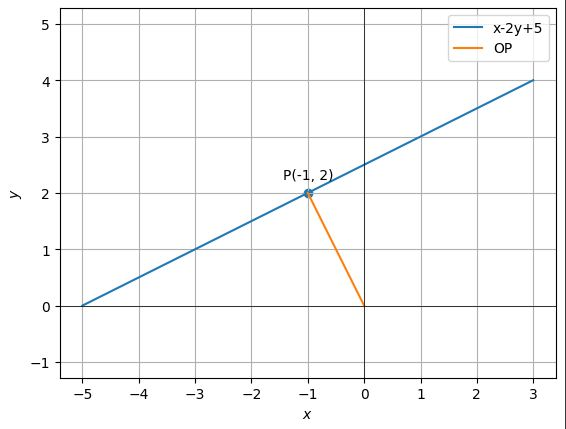
\includegraphics[width=1 \columnwidth]{graph.jpg}\\
	\caption{Graph}
	\label{fig:pic}
\end{figure}
 
\end{document}


